%Đây là template dùng cho đề cương đề tài tốt nghiệp
%Khoa Công nghệ Thông tin
%Trường Đại học Khoa học Tự nhiên, ĐHQG-HCM

%Liên hệ về mẫu LaTEX này: Thầy Bùi Huy Thông (bhthong@fit.hcmus.edu.vn)

\documentclass[14pt]{article}
\usepackage[utf8]{vietnam}
\usepackage{enumerate}
\usepackage{enumitem}
\usepackage{multicol}
\usepackage{listings}
\usepackage[left=3cm,right=2cm,top=2.5cm,bottom=2.5cm]{geometry}
\usepackage{verbatim}
\usepackage{graphicx}
\usepackage{url}
\usepackage{fancyhdr}
\usepackage{fancybox,framed}
\usepackage{xcolor}
\usepackage{array}
\usepackage{amsmath}
\usepackage{algorithm}
\usepackage{algorithmic}
\usepackage{lastpage}
\usepackage{float}
\usepackage{blindtext}
\usepackage{titlesec}
\usepackage[nottoc]{tocbibind}
\usepackage{setspace}
\usepackage{parskip}
\usepackage[colorlinks=true, linkcolor=blue!60!black, citecolor=blue!60!black, urlcolor=blue!60!black]{hyperref}


% -----------------------------------------------
% Giãn dòng và khoảng cách đoạn văn
% -----------------------------------------------
\setstretch{1.3}
\setlength{\parskip}{6pt}
\setlength{\parindent}{0.5cm}

% -----------------------------------------------
% Định dạng tiêu đề mục (section/subsection/subsubsection)
% -----------------------------------------------
\titleformat{\section}
  {\normalfont\fontsize{14pt}{17pt}\bfseries\MakeUppercase}
  {\thesection.}{0.5em}{}
\titlespacing*{\section}{0pt}{18pt}{8pt}

\titleformat{\subsection}
  {\normalfont\fontsize{13pt}{16pt}\bfseries}
  {\thesubsection.}{0.5em}{}
\titlespacing*{\subsection}{0pt}{14pt}{6pt}

\titleformat{\subsubsection}
  {\normalfont\fontsize{12pt}{15pt}\bfseries\itshape}
  {\thesubsubsection.}{0.5em}{}
\titlespacing*{\subsubsection}{0pt}{10pt}{4pt}

% -----------------------------------------------
% Header / Footer
% -----------------------------------------------
\pagestyle{fancy}
\fancyhf{}
\renewcommand{\headrulewidth}{0.4pt}
\renewcommand{\footrulewidth}{0.4pt}
\fancyhead[L]{\small\textit{Đề cương Khoá luận Tốt nghiệp}}
\fancyhead[R]{\small\textit{Khoa Công nghệ Thông tin -- HCMUS}}
\fancyfoot[C]{\small Trang \thepage\ / \pageref{LastPage}}

\pagenumbering{arabic}

% -----------------------------------------------
% Cỡ chữ mặc định toàn tài liệu: 12pt (tương đương \normalsize với base 14pt)
% -----------------------------------------------
\renewcommand{\normalsize}{\fontsize{12pt}{15pt}\selectfont}
\normalsize

\begin{document}

% ===============================================
% TRANG BÌA / HEADER THÔNG TIN
% ===============================================
\thispagestyle{empty}

\vfill

\begin{center}
    \textbf{\Large ĐẠI HỌC QUỐC GIA TP. HỒ CHÍ MINH}\\[5pt]
    \textbf{\Large TRƯỜNG ĐẠI HỌC KHOA HỌC TỰ NHIÊN}\\[5pt]
    \textbf{\Large KHOA CÔNG NGHỆ THÔNG TIN}
\end{center}

\vfill
\begin{center}
        
\includegraphics[scale=4]{logo2.png}
\end{center}
\vfill

\begin{center}
    \rule{\textwidth}{1.2pt}\\[10pt]
    {\fontsize{17pt}{21pt}\selectfont\textbf{ĐỀ CƯƠNG KHOÁ LUẬN TỐT NGHIỆP}}\\[10pt]
    \rule{\textwidth}{1.2pt}
\end{center}

\vfill

\begin{center}
    {\fontsize{13pt}{22pt}\selectfont\textbf{THIẾT KẾ VÀ ĐÁNH GIÁ CÁC CHIẾN LƯỢC TỰ ĐỘNG MỞ RỘNG\\[4pt]
    CHO CÁC HỆ THỐNG DỰA TRÊN KIẾN TRÚC MICROSERVICES}}\\[12pt]
    \textit{\normalsize (Design and Evaluation of Auto-scaling Strategies for Microservice-based Systems)}
\end{center}

\vfill

\begin{center}
    \rule{0.4\textwidth}{0.4pt}\\[6pt]
    \textit{TP. Hồ Chí Minh, năm 2026}
\end{center}

\vfill

\pagebreak

% ===============================================
% NỘI DUNG CHÍNH
% ===============================================

\section{THÔNG TIN CHUNG}

\begin{itemize}[leftmargin=1.5cm, label=\textbullet]
    \item \textbf{Người hướng dẫn:}
    \begin{itemize}[label=--]
        \item TS. Ngô Huy Biên (Khoa Công nghệ Thông tin, HCMUS)
    \end{itemize}

    \item \textbf{Sinh viên thực hiện:}
    \begin{enumerate}[label=\arabic*.]
        \item Nguyễn Quốc Khánh (MSSV: 22127188)
        \item Nguyễn Quang Khải (MSSV: 22127477)
    \end{enumerate}

    \item \textbf{Loại đề tài:} Nghiên cứu

    \item \textbf{Thời gian thực hiện:} Từ \textit{01/2026} đến \textit{07/2026}
\end{itemize}

\section{NỘI DUNG THỰC HIỆN}

\subsection{Giới thiệu về đề tài}

Kiến trúc Microservices cho phép các nhóm phát triển xây dựng và triển khai từng dịch vụ một cách độc lập, nhưng đồng thời đặt ra thách thức lớn trong việc đảm bảo khả năng co giãn. Trong các hệ thống thương mại điện tử -- chẳng hạn ứng dụng mẫu Google Online Boutique\footnote{\url{https://github.com/GoogleCloudPlatform/microservices-demo}} \cite{google2020boutique} -- lưu lượng truy cập có thể tăng đột biến (Flash Crowds), đạt mức 10.000 yêu cầu trong vài phút. Khi đó, nếu không có cơ chế tự động mở rộng phù hợp, thời gian phản hồi (Response Time) sẽ tăng vọt vượt ngưỡng cho phép, ảnh hưởng nghiêm trọng đến trải nghiệm người dùng và có thể gây ra sự cố sụp đổ dây chuyền.

Do đó, bài toán đặt ra là xây dựng một cơ chế tự động theo dõi và cấp phát tài nguyên có khả năng phản ứng nhanh, giữ độ trễ trong mức ổn định mà không lãng phí quá nhiều phần cứng.

\begin{figure}[H]
    \centering
    \vspace{0.5cm}
    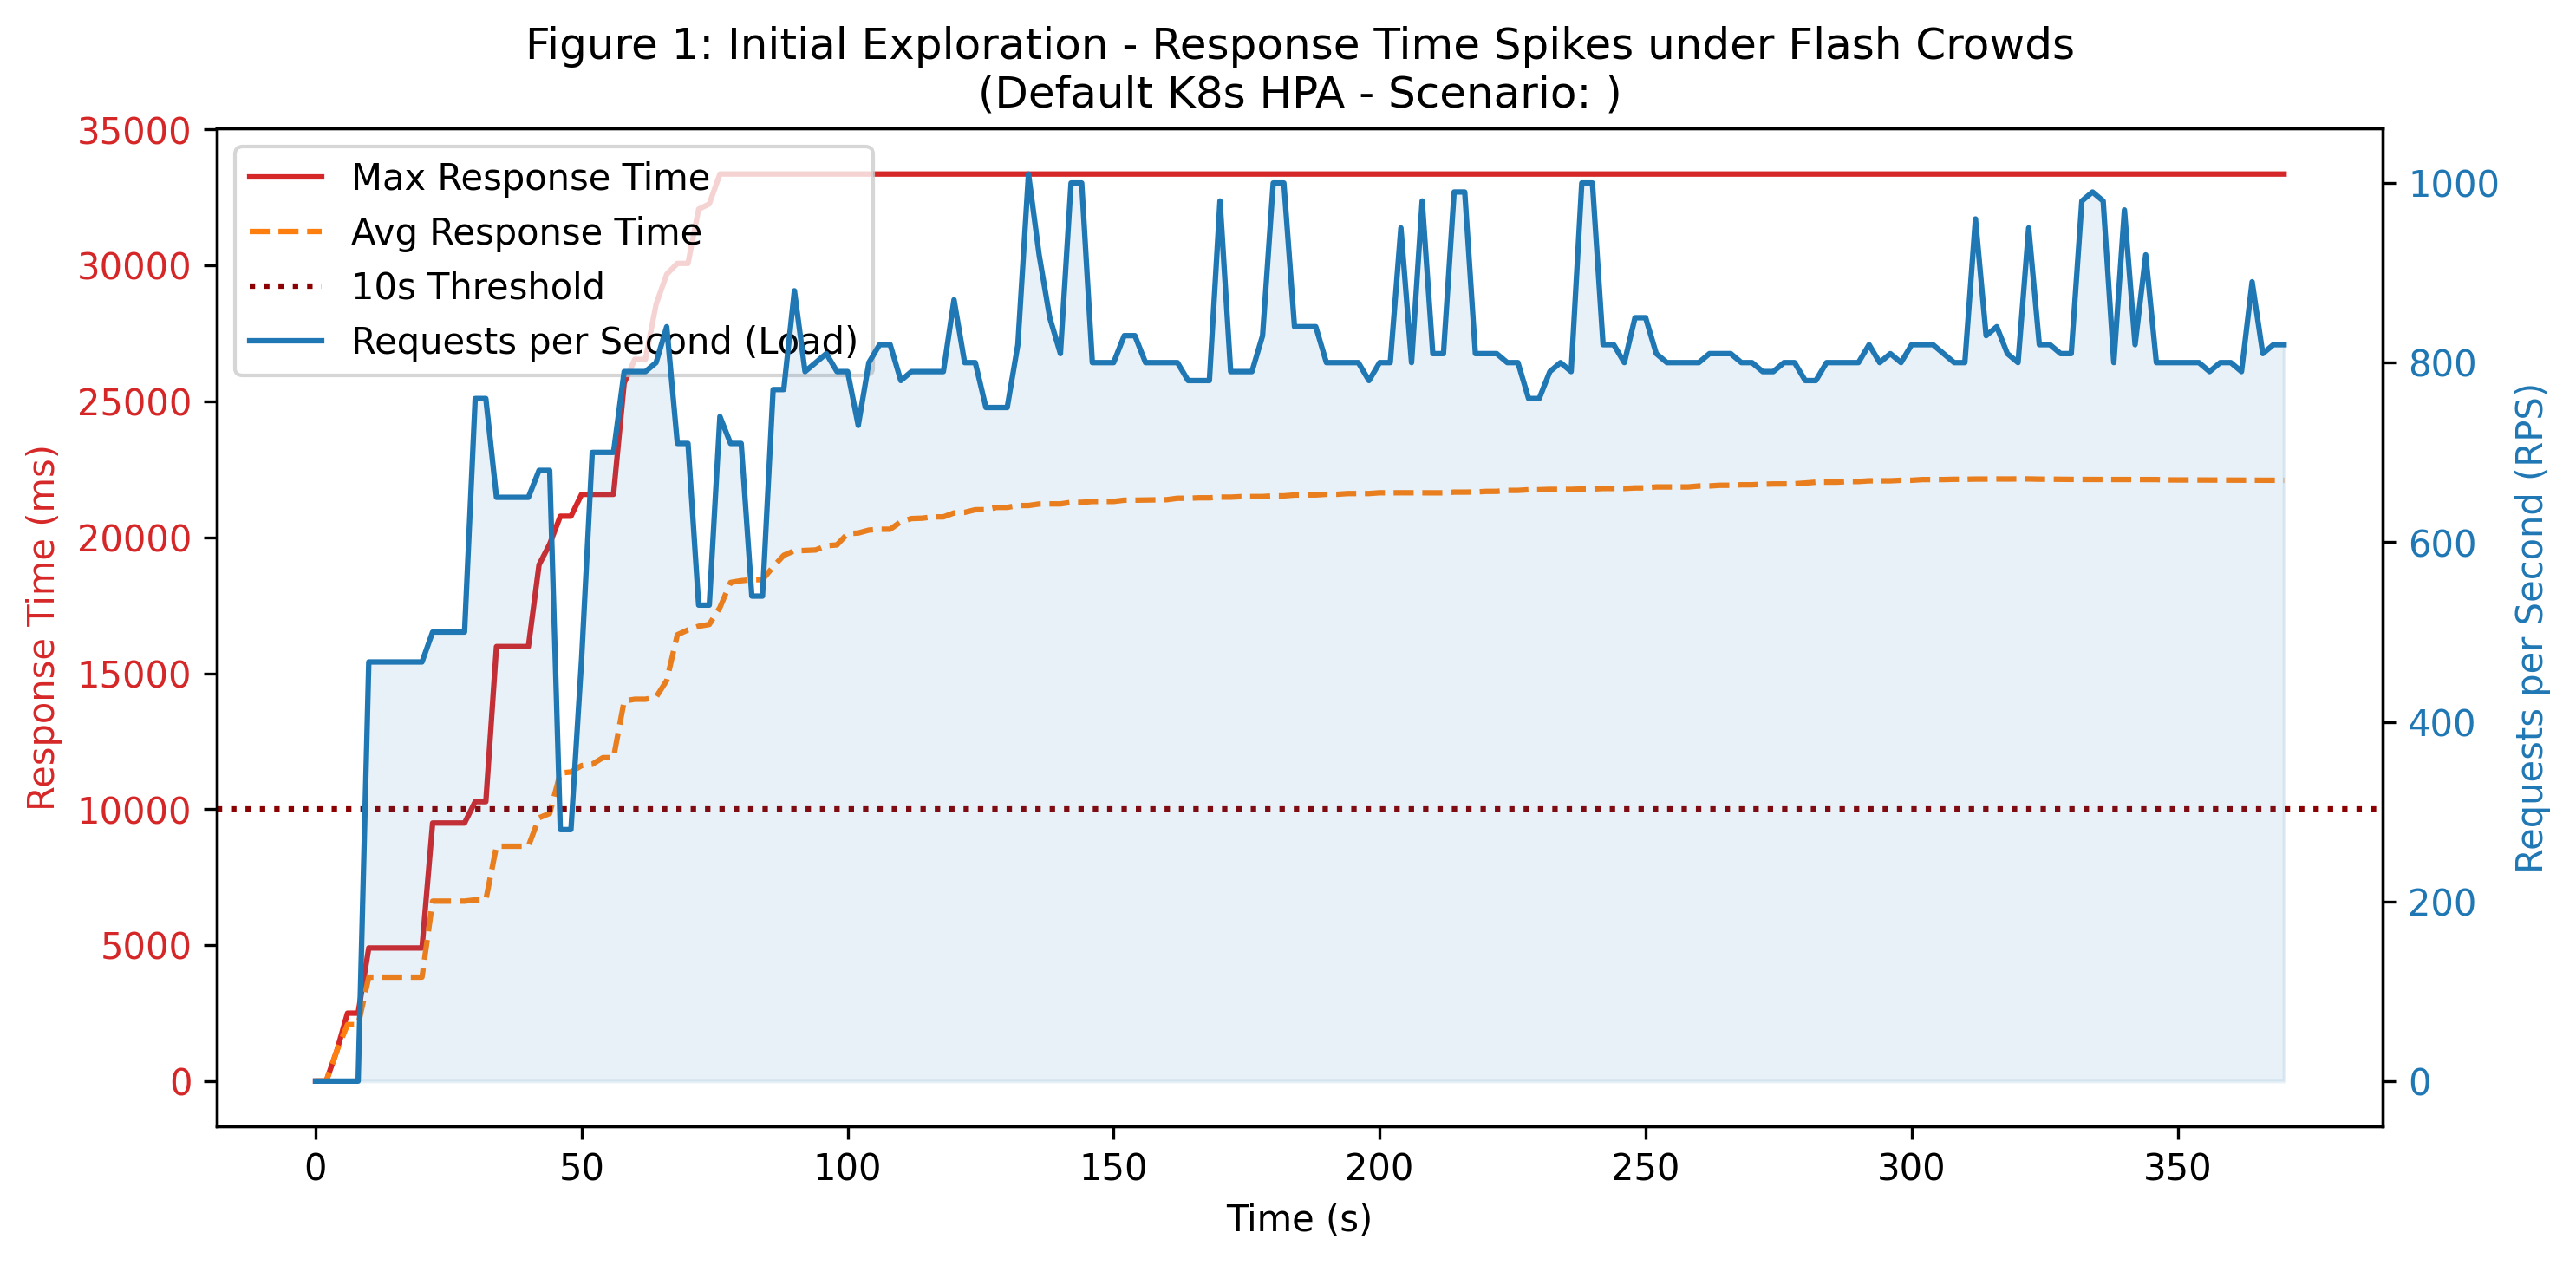
\includegraphics[width=0.85\textwidth]{images/figure1_problem_statement.png}
    \caption{Kết quả thăm dò ban đầu: Response Time tăng đột biến khi sử dụng K8s HPA mặc định dưới tải Flash Crowds.}
    \label{fig:figure1_problem_statement}
    \vspace{0.2cm}
\end{figure}

Hình~\ref{fig:figure1_problem_statement} minh họa vấn đề này: khi sử dụng Kubernetes HPA mặc định, Response Time tăng lên trên 10 giây trong các đợt Flash Crowds do hệ thống chỉ mở rộng \textit{sau khi} quá tải đã xảy ra. Từ bài toán thực tiễn này, đề tài đề xuất nghiên cứu và xây dựng \textbf{FlowSmart HPA} -- một cơ chế auto-scaling kết hợp dự báo chủ động với kiểm soát tải -- đồng thời tiến hành so sánh thực nghiệm với các giải pháp hiện có để đưa ra khuyến nghị phù hợp cho từng bối cảnh cụ thể.

\subsection{Nghiên cứu liên quan}

Hiện nay có nhiều giải pháp auto-scaling cho hệ thống microservices, mỗi giải pháp tiếp cận bài toán theo một hướng khác nhau. Dưới đây là các nghiên cứu liên quan chính mà đề tài sử dụng để so sánh và đối chiếu.

\subsubsection{Kubernetes HPA}

Kubernetes HPA là cơ chế auto-scaling mặc định, hoạt động theo nguyên lý đánh giá ngưỡng tĩnh để đối phó bị động với tải. HPA giám sát các chỉ số tài nguyên (CPU, RAM) thông qua \texttt{cgroups}, và tự động tăng/giảm số lượng Pod khi vượt ngưỡng cấu hình. Ưu điểm là đơn giản, có sẵn trong mọi cụm Kubernetes. Tuy nhiên, nhược điểm lớn nhất là tính thụ động: hệ thống chỉ mở rộng \textit{sau khi} quá tải đã xảy ra, dẫn đến phản ứng chậm trước các đợt tải đột biến.

\subsubsection{DeepScaler}

DeepScaler \cite{meng2023deepscaler} tiếp cận auto-scaling bằng mạng nơ-ron đồ thị (GNN) với khả năng phân tích biểu đồ phụ thuộc giữa các microservices. Thay vì xem xét từng dịch vụ riêng lẻ, DeepScaler phân loại mối quan hệ thời gian - không gian để đưa ra quyết định mở rộng đồng bộ cho những thành phần quan trọng. Giải pháp này cho hiệu năng tốt nhưng đòi hỏi phần cứng GPU để huấn luyện và suy luận, gây ra rào cản chi phí lớn cho các môi trường thực tế bị giới hạn ngân sách.

\subsubsection{GraphOpticon}

GraphOpticon \cite{theodoropoulos2026graphopticon} cũng sử dụng GNN nhưng có tính chất phân tích tải chặn trước ở phạm vi toàn hệ thống. Tương tự như DeepScaler, GraphOpticon cũng tiêu thụ tài nguyên GPU cho đồ thị mạng dữ liệu, khiến quá trình triển khai gặp rào cản về hạ tầng máy chủ.

\subsubsection{ProSmartHPA}

ProSmartHPA\footnote{\url{https://github.com/HussainAhmad05/ProSmart_HPA}} \cite{ahmad2025towards} cải thiện tính thụ động của K8s HPA bằng cách sử dụng các mô hình dự báo chuỗi thời gian để phòng ngừa sớm việc đột biến tải. Theo đó, mỗi dịch vụ microservice đều được gắn riêng một mô hình dự đoán xu hướng sử dụng tài nguyên của mình. Ưu điểm là không cần GPU, nhưng việc duy trì đồng thời nhiều tác vụ AI độc lập với nhau tạo ra khối block xử lý nặng và làm hao tổn phần cứng máy chủ quản lý.

\subsubsection{Tổng hợp so sánh}

\begin{table}[H]
\centering
\caption{So sánh ý tưởng cốt lõi của các giải pháp auto-scaling liên quan}
\renewcommand{\arraystretch}{1.3}
\begin{tabular}{|>{\raggedright\arraybackslash}p{2.8cm}|>{\raggedright\arraybackslash}p{3.2cm}|>{\raggedright\arraybackslash}p{3.5cm}|>{\raggedright\arraybackslash}p{4cm}|}
\hline
\textbf{Giải pháp} & \textbf{Cơ chế chính} & \textbf{Ưu điểm} & \textbf{Hạn chế} \\ \hline
K8s HPA & Reactive, đo CPU/RAM qua \texttt{cgroups} & Đơn giản, có sẵn & Phản ứng chậm, thụ động \\ \hline
DeepScaler & GNN phân tích đồ thị phụ thuộc & Scaling toàn diện, chính xác & Cần GPU, chi phí cao \\ \hline
GraphOpticon & GNN dự đoán toàn cục & Chủ động, phạm vi toàn cục & Cần GPU, chi phí cao \\ \hline
ProSmartHPA & Dự báo time-series cho từng dịch vụ & Chủ động, không cần GPU & Overhead cao do nhiều mô hình \\ \hline
\textbf{FlowSmart HPA} (đề xuất) & PROPHET + eBPF + Load Shedding & Chủ động, nhẹ, có cơ chế bảo vệ & \textit{Đang nghiên cứu} \\ \hline
\end{tabular}
\end{table}

\subsection{Mục tiêu đề tài}

\noindent\textbf{Vấn đề nghiên cứu:} Kubernetes HPA mặc định phản ứng chậm trước tải đột biến, dẫn đến quá tải hệ thống. Các giải pháp dựa trên Deep Learning (DeepScaler, GraphOpticon) cho hiệu năng tốt nhưng đòi hỏi GPU đắt đỏ. ProSmartHPA không cần GPU nhưng tạo ra overhead đáng kể do duy trì nhiều mô hình dự báo. Đề tài hướng đến việc xây dựng một giải pháp cân bằng giữa khả năng phản ứng nhanh và chi phí vận hành hợp lý.

\noindent\textbf{Tính cấp thiết:} Trong thực tế vận hành, lưu lượng truy cập tăng đột biến luôn là rủi ro hàng đầu đối với độ sẵn sàng của hệ thống. Các kỹ sư thường phải đối mặt với sự đánh đổi: cấu hình auto-scaling đơn giản thì phản ứng chậm, còn cấu hình phức tạp thì tiêu tốn nhiều tài nguyên. Đặc biệt trên các cụm máy chủ dùng chung, việc đảm bảo chất lượng dịch vụ càng khó khăn hơn do tình trạng tự tranh chấp lẫn nhau. Đề tài tập trung nghiên cứu bài toán này để tìm ra điểm cân bằng phù hợp trong kiến trúc microservices để không phải lãng phí đầu tư máy chủ.

\noindent\textbf{Mục tiêu nghiên cứu:} Đề tài đặt ra 4 mục tiêu cốt lõi:
\begin{itemize}[leftmargin=1.5cm, label=\textbullet]
    \item \textbf{(M1) Đề xuất giải pháp:} Xây dựng bộ điều khiển FlowSmart HPA (dưới dạng Kubernetes Operator) kết hợp mô hình dự báo PROPHET với công nghệ giám sát eBPF.
    \item \textbf{(M2) Tích hợp kiểm soát tải:} Áp dụng cơ chế Bounded Loads tại API Gateway để chủ động từ chối yêu cầu (Load Shedding) khi hệ thống đạt giới hạn tài nguyên, nhằm tối ưu lượng request thành công (Goodput) thay vì để hệ thống sụp đổ.
    \item \textbf{(M3) Thực nghiệm so sánh:} Thiết lập môi trường thử nghiệm trên Google Online Boutique, chạy các kịch bản tải (Flash Crowds, Spike, Ramp-up) để so sánh FlowSmart HPA với K8s HPA và ProSmartHPA.
    \item \textbf{(M4) Đánh giá và khuyến nghị:} Đo lường các chỉ số Response Time, Goodput, Control Plane Overhead để đánh giá khách quan và đưa ra khuyến nghị lựa chọn giải pháp phù hợp cho từng bối cảnh. Cung cấp mã nguồn mở và dữ liệu thực nghiệm.
\end{itemize}

\subsection{Phạm vi của đề tài}

\noindent\textbf{Đối tượng và công cụ nghiên cứu chính:}
\begin{itemize}[leftmargin=1.5cm, label=\textbullet]
    \item \textbf{FlowSmart HPA:} Bộ điều khiển tự động mở rộng chủ động do nhóm phát triển nghiên cứu (kết hợp PROPHET và eBPF).
    \item \textbf{Kubernetes HPA:} Cơ chế quản lý theo cụm gốc của Kubernetes, đóng vai trò hệ nhận chuẩn phản ứng thụ động cho thí nghiệm.
    \item \textbf{ProSmartHPA \cite{ahmad2025towards}:} Giải pháp tự động mở rộng theo thời gian, đóng vai trò là mẫu tham chiếu về chi phí vận hành thuật toán AI.
\end{itemize}

\noindent\textbf{Ứng dụng mẫu và Môi trường thực nghiệm:}
\begin{itemize}[leftmargin=1.5cm, label=\textbullet]
    \item \textbf{Ứng dụng mẫu:} Triển khai \textbf{Google Online Boutique} -- một hệ thống microservices dùng cho các bài thử nghiệm.
    \item \textbf{Môi trường:} Cụm Kubernetes trên Amazon EKS, liên tục khống chế ngân sách RAM và lõi xử lý để tái lập kịch bản khan hiếm cấu hình.
       \item \textbf{Giả lập tải:} Sử dụng framework mã nguồn mở \textbf{Locust}\footnote{\url{https://locust.io/}} để tạo làn sóng request theo biểu đồ giả định (như Flash Crowds).

\end{itemize}

\noindent\textbf{Giới hạn của đề tài:}
Để đảm bảo tính khả thi và tập trung vào mục tiêu giải quyết bài toán auto-scaling, các nội dung sau không thuộc phạm vi của Khóa luận:
\begin{itemize}[leftmargin=1.5cm, label=\textbullet]
    \item \textbf{Không sửa đổi logic ứng dụng:} Tôn trọng quy tắc "black-box", không chỉnh sửa mã nguồn nghiệp vụ của ứng dụng mẫu.
    \item \textbf{Không sử dụng Deep Learning/GNN:} Nhằm tối ưu hóa chi phí vận hành, đề tài chỉ giới hạn ở các mô hình thống kê hạng nhẹ, không sử dụng các mô hình AI đòi hỏi GPU.
    \item \textbf{Không đánh giá trải nghiệm người dùng chủ quan:} Toàn bộ hiệu năng được đo lường tự động bằng các chỉ số hệ thống kỹ thuật, không bao gồm khảo sát bằng survey.
    \item \textbf{Không can thiệp hạ tầng mạng lõi:} Không sửa đổi hệ điều khiển mạng cốt lõi (CNI) hay các cấu hình bảo mật chuyên sâu.
\end{itemize}

\subsection{Cách tiếp cận và Phương pháp thực nghiệm}

Cách tiếp cận của đề tài bao gồm hai giai đoạn: (1) Xây dựng giải pháp FlowSmart HPA và (2) Thực hiện các kịch bản thực nghiệm trên ứng dụng mẫu để so sánh, đánh giá và đưa ra khuyến nghị thực tiễn.

\subsubsection{Kiến trúc giải pháp FlowSmart HPA}

Thay vì chỉ giám sát các chỉ số tài nguyên một cách thụ động, FlowSmart HPA tiếp cận theo hướng kết hợp (Hybrid), bao gồm 3 thành phần cốt lõi:
\begin{itemize}[leftmargin=1.5cm, label=\textbullet]
    \item \textbf{Predictive Ingress Monitor:} Sử dụng mô hình thống kê chuỗi thời gian PROPHET\footnote{\url{https://facebook.github.io/prophet/}} \cite{taylor2018forecasting} để dự báo trước tải trọng tại cổng vào (API Gateway), giúp mở rộng Pod trước khi xảy ra nghẽn.
    \item \textbf{Topology-aware Priority Allocator:} Khai thác công nghệ eBPF ở tầng nhân (kernel) để theo dõi các luồng giao tiếp mạng giữa các microservices, từ đó định tuyến tài nguyên ưu tiên cho các dịch vụ cốt lõi.
    \item \textbf{Bounded Loads Enforcer:} Cơ chế kiểm soát tải tại API Gateway. Khi hệ thống đạt giới hạn tài nguyên, Gateway sẽ chủ động từ chối (Load Shedding) các yêu cầu vượt ngưỡng để bảo vệ cụm \cite{mirrokni2017consistent}.
\end{itemize}

\begin{figure}[H]
    \centering
    \vspace{0.5cm}
    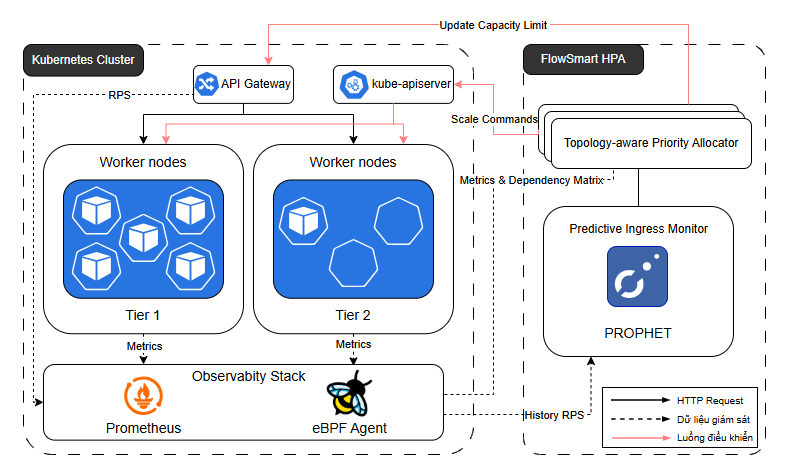
\includegraphics[width=0.85\textwidth]{images/system_architecture.png}
    \caption{Sơ đồ khối các thành phần và luồng tương tác của hệ thống FlowSmart HPA.}
    \label{fig:block_diagram}
\end{figure}

\subsubsection{Mô hình hóa toán học bài toán Scaling}

Hệ thống sử dụng đại số tuyến tính để nội suy nhu cầu tài nguyên lý tưởng dựa trên giá trị $C_{knee}$ (ngưỡng lưu lượng tối đa một Pod có thể xử lý trước khi suy thoái phi tuyến tính):
\begin{equation}
    \mathrm{Pod}_{\mathrm{ideal}, i} = \left\lceil \frac{\hat{\lambda}_{gw} \times w_i}{C_{knee, i} \times \mu_{\mathrm{target}}} \right\rceil
\end{equation}

Khi tổng nhu cầu vượt quá ngân sách $B$ ($\sum \mathrm{Pod}_{\mathrm{ideal}, i} > B$), hệ thống phân bổ lại theo trọng số Critical Path Prioritization ($P_{path, i}$) \cite{xie2024pbscaler}:
\begin{equation}
    \mathrm{Pod}_{\mathrm{actual}, i} = \left\lfloor B \times \frac{\mathrm{Pod}_{\mathrm{ideal}, i} \times P_{path, i}}{\sum_{j=1}^{N} (\mathrm{Pod}_{\mathrm{ideal}, j} \times P_{path, j})} \right\rfloor
\end{equation}

\begin{algorithm}[H]
\caption{FlowSmart Global Scaling Strategy}
\label{alg:flowsmart}
\begin{algorithmic}[1]
\renewcommand{\algorithmicrequire}{\textbf{Input:}}
\renewcommand{\algorithmicensure}{\textbf{Output:}}
\REQUIRE $\mathcal{S}$; $B$; $\mathcal{H}_{gw}$; $\mathbf{M}$ (trích xuất qua eBPF); $C_{knee}$; $P_{path}$;
\ENSURE $\mathcal{A}$ (Replicas); $\mathcal{L}_{gw}$ (Rate-limit);

\STATE \textbf{Bước 1:} $\hat{\lambda}_{gw} \leftarrow \text{Prophet}(\mathcal{H}_{gw})$ \COMMENT{Dự báo lưu lượng}
\STATE \textbf{Bước 2: Tính nhu cầu lý tưởng}
\FORALL{$s_i \in \mathcal{S}$}
    \STATE $w_i \leftarrow$ Trích xuất hệ số lan truyền từ $\mathbf{M}$
    \STATE $r_i \leftarrow \lceil (\hat{\lambda}_{gw} \times w_i) / (C_{knee,i} \times U_{target}) \rceil$
\ENDFOR
\STATE \textbf{Bước 3: Phân bổ tài nguyên thực tế}
\IF{$\sum r_i \le B$}
    \STATE $\mathcal{A} \leftarrow \{r_1, ..., r_n\}$
\ELSE
    \STATE $D \leftarrow \sum (r_j \times P_{path,j})$
    \FORALL{$s_i \in \mathcal{S}$}
        \STATE $a_i \leftarrow \lfloor B \times (r_i \times P_{path,i}) / D \rfloor$
    \ENDFOR
    \STATE $\mathcal{A} \leftarrow \{a_1, ..., a_n\}$
\ENDIF
\STATE \textbf{Bước 4: Thực thi và Phòng vệ}
\STATE $\mathcal{L}_{gw} \leftarrow \min_{i \in \text{CorePaths}} (a_i \times C_{knee,i} / w_i)$ \COMMENT{Tính giới hạn an toàn}
\STATE Cập nhật $\mathcal{A}$ lên K8s API và $\mathcal{L}_{gw}$ lên API Gateway
\RETURN $\mathcal{A}$
\end{algorithmic}
\end{algorithm}

\subsubsection{Cấu hình môi trường thực nghiệm và Phân định công việc}

Để đảm bảo kết quả đánh giá khách quan và công bằng, đồng thời phân định rõ giữa các công cụ có sẵn và các thành phần tự phát triển, đề tài được tổ chức như sau:

\begin{itemize}[leftmargin=1.5cm, label=\textbullet]
    \item \textbf{(1) Khối công cụ nền tảng và Môi trường tham chiếu (Đã có sẵn):}
    \begin{itemize}[label=--]
        \item \textit{Hạ tầng Máy chủ (Cluster Topology):} Cụm Amazon EKS giới hạn với 3 Worker Nodes (cấu hình \texttt{c7i.flex-large}: 2 vCPU, 4GB RAM/Node) nhằm ép hệ thống dễ dàng chạm trần và sinh ra điểm nghẽn.
        \item \textit{Ứng dụng mẫu (Microservices Limits):} Sử dụng Google Online Boutique với các Core Pods (\texttt{frontend}, \texttt{cartservice}) bị giới hạn tài nguyên ở mức CPU 200m và 256Mi Memory để tạo điểm nghẽn chuẩn (Knee-point).
        \item \textit{Công cụ giám sát \& Baseline:} Sử dụng K8s HPA mặc định và mã nguồn mở ProSmartHPA làm baseline; kết hợp Prometheus/Grafana để thu thập, trực quan hóa thông số.
        \item \textit{Tham số Bơm tải (Workload Generator):} Cấu hình Locust mô phỏng tải dựa trên dữ liệu thực tế (Real-world HTTP traces) như \textbf{WorldCup98 logs} hay \textbf{NASA logs}, sử dụng đúng bộ dữ liệu chuẩn của nghiên cứu Baseline \cite{ahmad2025towards}.
    \end{itemize}

    \begin{figure}[H]
        \centering
        \vspace{0.5cm}
        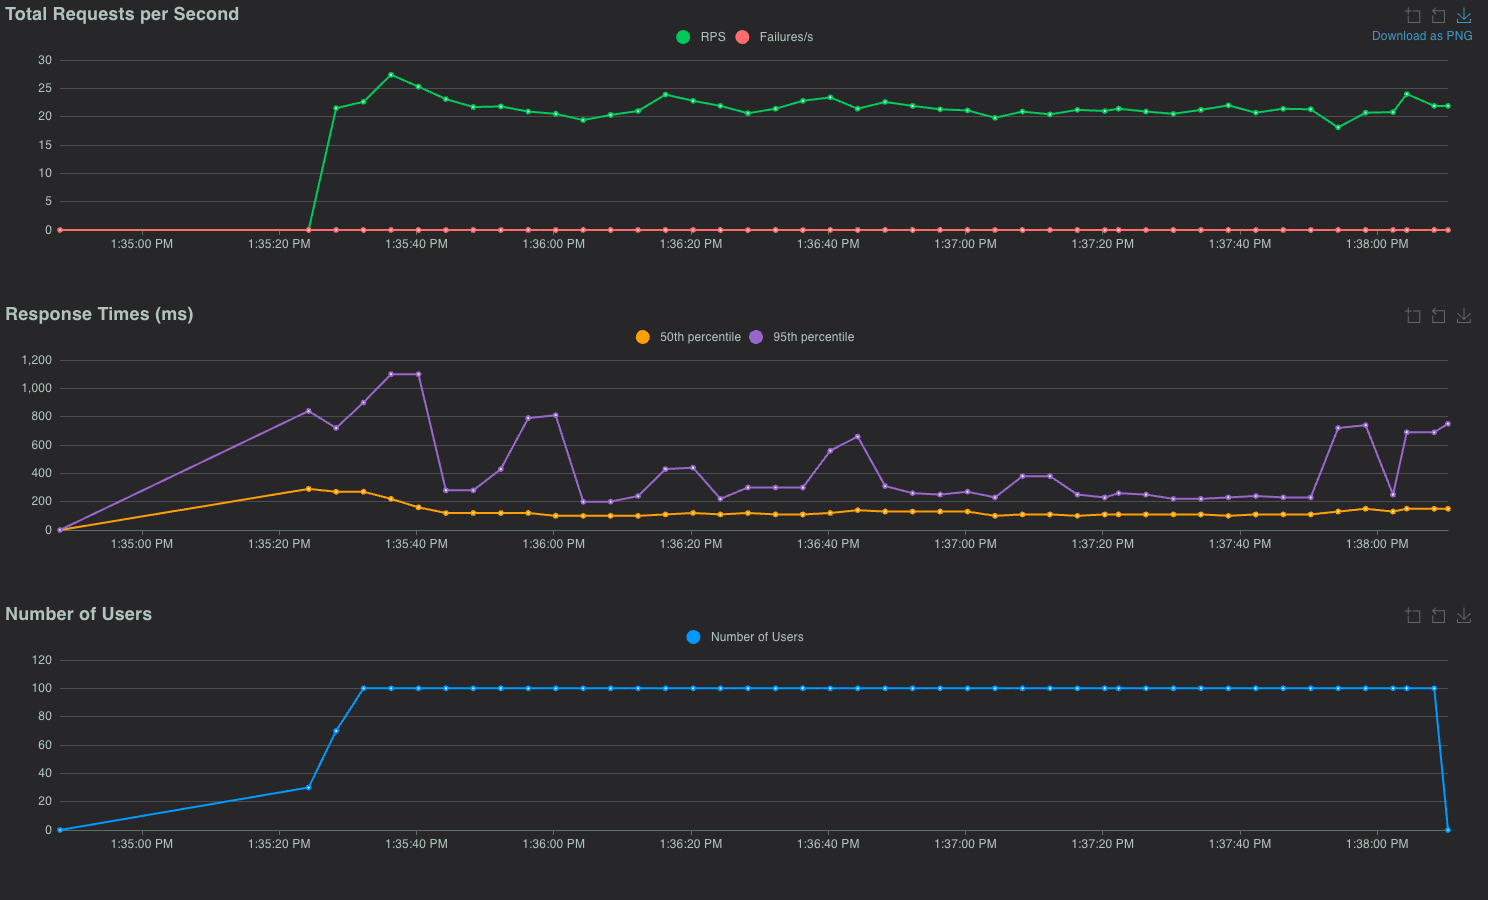
\includegraphics[width=0.85\textwidth]{images/locust_env_proof.png}
        \caption{ Giao diện công cụ giả lập tải Locust được thiết lập để chuẩn bị cho các kịch bản thực nghiệm.}
        \label{fig:env_proof}
        \vspace{0.2cm}
    \end{figure}

    \item \textbf{(2) Khối lượng công việc cốt lõi (Sẽ nghiên cứu \& lập trình mới):}
    \begin{itemize}[label=--]
        \item \textit{Phát triển Controller trung tâm:} Thiết kế kiến trúc và lập trình khối điều khiển \textbf{FlowSmart Operator} hoàn chỉnh bằng ngôn ngữ Python, tích hợp sâu vào API điều phối của Kubernetes (Custom Resource Definition).
        \item \textit{Cấu trúc module giám sát eBPF:} Khảo sát và biên dịch các tệp lệnh eBPF (ngôn ngữ C) lồng vào tầng nhân (kernel Linux) để lọc và thu thập dữ liệu lưu lượng microservices với chi phí Overhead cực kỳ nhỏ.
        \item \textit{Khớp nối mô hình \& Giải thuật xử lý:} Tự lập trình module tích hợp đẩy dữ liệu eBPF qua mô hình PROPHET theo chuỗi thời gian thực (Real-time streaming). Đồng thời tự hiện thực cơ chế kiểm soát tải (Bounded Loads) tại Ingress API Gateway để bảo vệ hệ thống khỏi sụp đổ.
    \end{itemize}
\end{itemize}

\subsubsection{Thiết kế Kịch bản Thực nghiệm (Đánh giá các bài toán chuyên biệt)}

Dựa trên cấu hình bối cảnh đã tham chiếu kể trên, nghiên cứu đi vào đo lường thực tiễn với 4 chuỗi thực nghiệm. Mục tiêu là cô lập và đánh giá hiệu năng của 3 hệ thống (K8s HPA tiêu chuẩn, ProSmartHPA, và FlowSmart HPA).

\begin{itemize}[leftmargin=1.5cm, label=\textbullet]
    \item \textbf{TN1: Đánh giá độ trễ dưới đợt tải truy cập đột biến (Flash Crowds)}
    \begin{itemize}[label=--]
        \item \textit{Vấn đề:} Khi lượng requests tăng vọt từ 100 lên 5.000 RPS trong 1 phút, hệ thống có giữ được thời gian phản hồi ổn định không?
        \item \textit{Cách tiến hành:} Dùng Locust bơm tải theo kịch bản Spike. Đo lường Response Time (thời gian phản hồi trung bình và p99) cùng Tỷ lệ vi phạm SLO.
        \item \textit{Kỳ vọng:} K8s HPA dự kiến có Response Time cao (> 10s) do phản ứng chậm. ProSmartHPA và FlowSmart HPA kỳ vọng phản ứng nhanh hơn nhờ cơ chế dự báo, tuy nhiên mức cải thiện cụ thể sẽ được xác nhận qua thực nghiệm.
    \end{itemize}
    
    \item \textbf{TN2: Đánh giá khả năng chịu tải khi hệ thống cạn kiệt tài nguyên vật lý (Under-provisioning)}
    \begin{itemize}[label=--]
        \item \textit{Vấn đề:} Khi cụm Kubernetes bị khóa giới hạn tối đa phần cứng nhưng tải vẫn tiếp tục tăng, hệ thống sẽ phản ứng thế nào?
        \item \textit{Cách tiến hành:} Đẩy tải vượt quá khả năng chịu đựng của phần cứng vật lý. Đo lường chỉ số \textbf{Goodput} (tổng lượng yêu cầu được xử lý thành công với mã 200 OK).
        \item \textit{Kỳ vọng:} K8s HPA không có cơ chế bảo vệ nên có nguy cơ sụp đổ toàn cụm (Cascading Failure), khiến Goodput giảm mạnh. FlowSmart HPA kỳ vọng duy trì Goodput ổn định nhờ cơ chế Load Shedding, tuy hiệu quả thực tế phụ thuộc vào cấu hình ngưỡng.
    \end{itemize}

    \item \textbf{TN3: Đánh giá chi phí vận hành hệ thống điều khiển (Control Plane Overhead)}
    \begin{itemize}[label=--]
        \item \textit{Vấn đề:} Hệ thống Auto-scaling có tiêu tốn quá nhiều tài nguyên của cụm để tự vận hành các thuật toán AI của nó hay không?
        \item \textit{Cách tiến hành:} Đo lường lượng CPU và RAM tiêu thụ của bản thân Controller trong quá trình hoạt động.
        \item \textit{Kỳ vọng:} K8s HPA dự kiến tiêu thụ ít tài nguyên nhất do cơ chế đơn giản. FlowSmart HPA kỳ vọng tiêu thụ ít hơn ProSmartHPA nhờ chỉ sử dụng một mô hình dự báo duy nhất thay vì nhiều mô hình độc lập.
    \end{itemize}

    \item \textbf{TN4: Đánh giá năng lực thu hồi tài nguyên dưới tải dao động (Sinusoidal Load)}
    \begin{itemize}[label=--]
        \item \textit{Vấn đề:} Khi lưu lượng người dùng tăng giảm liên tục theo chu kỳ (ví dụ: chu kỳ theo ngày/đêm), hệ thống có giải phóng tài nguyên đủ nhanh khi tải xuống thấp để tránh lãng phí (Over-provisioning) hay không?
        \item \textit{Cách tiến hành:} Bơm tải theo mô hình hình sin (tăng/giảm liên tục) bằng Locust. Đo lường tỷ lệ Pod nhàn rỗi được duy trì và độ trễ thu hồi tài nguyên.
        \item \textit{Kỳ vọng:} ProSmartHPA và FlowSmart HPA kỳ vọng nhận diện chu kỳ tải tốt hơn K8s HPA nhờ khả năng dự báo. Mức độ tiết kiệm tài nguyên cụ thể giữa các giải pháp sẽ được xác nhận qua thực nghiệm.
    \end{itemize}

\end{itemize}

\subsubsection{Khung đánh giá tổng hợp và Khuyến nghị}

Từ dữ liệu thu thập được ở các kịch bản thực nghiệm, đề tài sẽ đánh giá hiệu năng tổng thể thông qua bộ chỉ số đo lường hiệu suất tài nguyên (Resource Efficiency). Từ đó, kết quả nghiên cứu sẽ được đúc kết thành một \textbf{Ma trận quyết định chiến lược Auto-scaling} để trực quan hóa hướng dẫn dành cho các kỹ sư hệ thống. Bảng~\ref{table:decision_matrix_mock} phác thảo cấu trúc dự kiến của ma trận này.

\begin{table}[H]
\centering
\caption{Cấu trúc dự kiến của Ma trận quyết định chiến lược Auto-scaling}
\label{table:decision_matrix_mock}
\renewcommand{\arraystretch}{1.4}
\begin{tabular}{|>{\raggedright\arraybackslash}p{4cm}|>{\centering\arraybackslash}p{3.5cm}|>{\centering\arraybackslash}p{3.5cm}|>{\centering\arraybackslash}p{3.5cm}|}
\hline
\textbf{Kịch bản / Yêu cầu} & \textbf{K8s HPA} & \textbf{ProSmartHPA} & \textbf{FlowSmart HPA} \\ \hline
Tải đột biến, cần Response Time thấp & Chậm phản ứng & Dự báo sát & Dự báo + Bảo vệ \\ \hline
Tài nguyên phần cứng hạn chế & Dễ sụp đổ cụm & Tải nặng máy chủ & Chủ động loại tải \\ \hline
Mục tiêu tiết kiệm tài nguyên quản lý & Rất nhẹ & Quá tải mô hình & Chỉ một mô hình AI \\ \hline
Độ dễ dàng cho hạ tầng & Tích hợp sẵn & Cần cấu hình chéo & Phức tạp (nhúng eBPF) \\ \hline
\end{tabular}
\end{table}

\subsection{Kết quả dự kiến của đề tài}

Sau quá trình nghiên cứu, xây dựng và thực nghiệm, đề tài hướng đến các kết quả cụ thể trên ba phương diện: số liệu định lượng, sản phẩm phần mềm và tài liệu kỹ thuật.

\subsubsection{Số liệu định lượng mục tiêu (Evaluation Metrics)}

\begin{table}[H]
\centering
\caption{Các chỉ số định lượng mục tiêu}
\renewcommand{\arraystretch}{1.3}
\begin{tabular}{|>{\raggedright\arraybackslash}p{4.5cm}|>{\raggedright\arraybackslash}p{5cm}|>{\raggedright\arraybackslash}p{5cm}|}
\hline
\textbf{Chỉ số đo lường} & \textbf{Định nghĩa} & \textbf{Mục tiêu / Kỳ vọng} \\ \hline
\textbf{Response Time} & Thời gian trung bình và p99 để xử lý 1 request. & Duy trì ổn định dưới 2s khi gặp tải đột biến (Spike Load). \\ \hline
\textbf{Goodput} & Tổng số request được xử lý thành công (mã HTTP 200 OK). & Đi ngang và duy trì ở mức tối đa của phần cứng khi bị quá tải. \\ \hline
\textbf{Error Rate} & Tỷ lệ request trả về lỗi sập nguồn (502, 504) hoặc timeout. & Thấp hơn đáng kể so với K8s HPA nhờ cơ chế chủ động từ chối. \\ \hline
\textbf{Control Plane Overhead} & Lượng CPU/RAM mà bản thân bộ điều khiển tiêu thụ. & Đạt mức tiết kiệm tài nguyên tương đương K8s HPA, thấp hơn 60\% so với ProSmartHPA. \\ \hline
\textbf{REI Score} & Điểm tổng hợp: Hiệu năng - Chi phí - Độ ổn định. & FlowSmart HPA đạt điểm REI cao nhất trong 3 hệ thống đánh giá. \\ \hline
\end{tabular}
\end{table}

\subsubsection{Sản phẩm phần mềm và Dữ liệu nghiên cứu}

\begin{itemize}[leftmargin=1.5cm, label=\textbullet]
    \item \textbf{FlowSmart Operator:} Bộ điều khiển tự động mở rộng hoàn chỉnh được đóng gói cho Kubernetes, lập trình bằng Python/Go, tích hợp sẵn mô hình PROPHET và agent eBPF.
    \item \textbf{Bộ kịch bản kiểm thử:} Các file kịch bản Locust giả lập tải (Spike, Flash Crowds) có thể chạy tự động để cộng đồng tái tạo thực nghiệm.
    \item \textbf{Ma trận quyết định chiến lược Auto-scaling:} Tài liệu đúc kết từ thực nghiệm, hướng dẫn chi tiết các kỹ sư khi nào nên dùng công cụ nào tương ứng với từng cấu hình bài toán cụ thể.
    \item \textbf{Tập dữ liệu hiệu năng (Dataset):} Các file CSV/JSON trích xuất từ Prometheus ghi lại độ trễ, CPU, RAM và số lượng Pod của 3 hệ thống qua từng giây thực nghiệm.
\end{itemize}

\subsection{Kế hoạch thực hiện}

Kế hoạch thực hiện được điều chỉnh bám sát các mốc thời gian của Khoa và tiến trình xây dựng, đánh giá 4 kịch bản thực nghiệm (TN1, TN2, TN3, TN4).

\begin{table}[H]
\centering
\caption{Kế hoạch thực hiện dự kiến}
\renewcommand{\arraystretch}{1.4}
\begin{tabular}{|>{\raggedright\arraybackslash}p{2.6cm}
                |>{\centering\arraybackslash}p{3.2cm}
                |>{\raggedright\arraybackslash}p{8.6cm}|}
\hline
\textbf{Thời gian} & \textbf{Trạng thái} & \textbf{Nội dung công việc} \\ \hline
19/10/2025
  & \textcolor{green!70!black}{Đã hoàn thành}
  & Ngày bắt đầu: Khoa thông báo chính thức về việc thực hiện đề tài khóa luận. \\ \hline
26/12/2025 
  & \textcolor{green!70!black}{Đã hoàn thành}
  & Ngày nộp đơn đăng ký: Nộp đơn đăng ký thực hiện đề tài về Khoa. \\ \hline
26/12/2025 -- 01/04/2026
  & \textcolor{green!70!black}{Đã hoàn thành}
  & Tìm hiểu bài báo và công nghệ: Nghiên cứu chuyên sâu về mô hình PROPHET, công nghệ trích xuất topology mạng eBPF, và cơ chế Bounded Loads. \\ \hline
04/04/2026
  & \textcolor{green!70!black}{Đã hoàn thành}
  & Ngày hiện tại: Mốc thời gian hiện tại. \\ \hline
06/04/2026
  & \textcolor{orange}{Đang tiến hành}
  & \textbf{Ngày nộp đề cương:} Hoàn thiện và nộp bản đề cương chi tiết đã hiệu chỉnh theo hướng thực nghiệm, giải quyết bài toán thực tế. \\ \hline
07/04 -- 15/06/2026
  & \textcolor{red}{Chưa thực hiện}
  & \textbf{Xây dựng giải pháp và Thực nghiệm (TN1, TN2, TN3):} Thiết lập cụm Kubernetes. Lập trình FlowSmart Operator. Bơm tải Flash Crowds bằng Locust. Đo lường Response Time, Goodput, và Overhead so với các Baselines. \\ \hline
01/06 -- 10/07/2026
  & \textcolor{red}{Chưa thực hiện}
  & \textbf{Viết báo cáo khóa luận:} Xây dựng Ma trận quyết định chiến lược Auto-scaling. Đóng gói mã nguồn. Tổng hợp cơ sở lý thuyết và phân tích số liệu thực nghiệm. \\ \hline
20/07/2026
  & \textcolor{red}{Chưa thực hiện}
  & Ngày kết thúc: Hoàn tất thủ tục nộp đơn đăng ký bảo vệ khóa luận trước hội đồng. \\ \hline
\end{tabular}
\end{table}

\pagebreak

% ===============================================
% TÀI LIỆU THAM KHẢO
% ===============================================
\renewcommand{\refname}{Tài liệu tham khảo}
\bibliographystyle{IEEEtran}
\bibliography{references}

\vspace{2cm}

% ===============================================
% KÝ TÊN
% ===============================================
\noindent
\begin{minipage}[t]{0.48\textwidth}
    \centering
    \textbf{XÁC NHẬN }\\[4pt]
    \textbf{CỦA NGƯỜI HƯỚNG DẪN}\\[4pt]
    \textit{(Ký và ghi rõ họ tên)}\vspace{3cm}

\end{minipage}%
\hfill
\begin{minipage}[t]{0.48\textwidth}
    \centering
    \textit{TP. Hồ Chí Minh, ngày \hspace{0.1cm} tháng \hspace{0.1cm} năm 2026}\\[4pt]
    \textbf{SINH VIÊN THỰC HIỆN}\\[4pt]
    \textit{(Ký và ghi rõ họ tên)}\\[3cm]
\end{minipage}

\end{document}